\documentclass[aspectratio=169,11pt]{beamer}
% ==========================================================================
%  KSA lecture-slide theme  =  stock beamer "Boadilla"  +  KSA colour theme
%  brand colours sampled from the official KSA symbol mark:
%    Deep Prussian Blue  #2E3192   (지성 - intellect)
%    Golden Gray         #D6CBB1   (감성 - sensibility)
%  Engine: XeLaTeX.  Usage:
%    \documentclass[aspectratio=169,11pt]{beamer}
%    \input{../../theme/ksa-theme.tex}
%  Each deck lives in its own slides/kor/<deck>/ folder together with its
%  own images; ../../figs/ is kept only as a fallback for the shared cache.
% ==========================================================================

\usepackage{fontspec}
\usepackage{amsmath,amssymb}
\usepackage{graphicx}
\graphicspath{{figs/}{./}{../../../figs/}}
\usepackage{booktabs}
\usepackage{listings}
\usepackage{varwidth}

% ---- fonts (no ctex/xeCJK on this box -> fontspec drives CJK directly) -----
\defaultfontfeatures{Ligatures=TeX}
\setmainfont{Noto Sans CJK KR}
\setsansfont{Noto Sans CJK KR}
\setmonofont{Noto Sans Mono CJK KR}[Scale=0.92]

% ---- base theme: stock Boadilla ------------------------------------------
\usetheme{Boadilla}
\usefonttheme{professionalfonts}
\setbeamertemplate{navigation symbols}{}

% ---- KSA colour theme (recolour the stock theme) --------------------------
\definecolor{ksablue}{HTML}{2E3192}
\definecolor{ksabluedk}{HTML}{20226A}
\definecolor{ksagold}{HTML}{D6CBB1}
\definecolor{ksagolddk}{HTML}{A9976B}
\definecolor{ksared}{HTML}{C0392B}
\definecolor{ksagray}{HTML}{5B5B5B}

\setbeamercolor{structure}{fg=ksablue}
\setbeamercolor{alerted text}{fg=ksared}

\setbeamercolor{palette primary}{fg=white,           bg=ksablue}
\setbeamercolor{palette secondary}{fg=white,         bg=ksablue!85!black}
\setbeamercolor{palette tertiary}{fg=white,          bg=ksabluedk}
\setbeamercolor{titlelike}{fg=ksablue}
\setbeamercolor{frametitle}{fg=ksablue,bg=}
\setbeamercolor{title}{fg=ksablue}
\setbeamercolor{author}{fg=ksagray}
\setbeamercolor{institute}{fg=ksagray}
\setbeamercolor{block title}{fg=white,bg=ksablue}
\setbeamercolor{block body}{fg=black!85,bg=ksablue!6}
\setbeamercolor{item}{fg=ksablue}
\setbeamercolor{section in toc}{fg=black!85}

\setbeamerfont{frametitle}{series=\bfseries}
\setbeamerfont{title}{series=\bfseries}

% ---- footline:  KSA mark | "Made by ..." | n / N   (matches reference) ----
\newcommand{\ksacredit}{}
\setbeamertemplate{footline}{%
  \hbox{%
    \begin{beamercolorbox}[wd=.18\paperwidth,ht=2.6ex,dp=1.5ex,leftskip=1.1em]{}%
      \raisebox{-0.35ex}{\includegraphics[height=2.0ex]{ksa-logo.png}}%
    \end{beamercolorbox}%
    \begin{beamercolorbox}[wd=.64\paperwidth,ht=2.6ex,dp=1.5ex,center]{}%
      {\scriptsize\color{ksagray}\ksacredit}%
    \end{beamercolorbox}%
    \begin{beamercolorbox}[wd=.18\paperwidth,ht=2.6ex,dp=1.5ex,rightskip=1.1em]{}%
      \hfill{\scriptsize\color{ksablue}\insertframenumber\,/\,\inserttotalframenumber}%
    \end{beamercolorbox}%
  }%
  \vskip2pt
}

% ---- section divider: stock \sectionpage, KSA-coloured -------------------
\setbeamertemplate{section page}{%
  \begingroup\centering
    {\color{ksagolddk}\rule{0.16\paperwidth}{1pt}}\par\vskip1.0em
    {\usebeamerfont{title}\color{ksablue}\insertsectionhead\par}\vskip1.0em
    {\color{ksagolddk}\rule{0.16\paperwidth}{1pt}}\par
  \endgroup
}
\AtBeginSection[]{\begin{frame}[plain,noframenumbering]\vfill\sectionpage\vfill\end{frame}}

% ---- code listings ------------------------------------------------------------
\lstdefinestyle{ksa}{%
  basicstyle=\ttfamily\scriptsize,
  keywordstyle=\color{ksablue}\bfseries,
  commentstyle=\color{ksagray}\itshape,
  stringstyle=\color{ksagolddk},
  numberstyle=\tiny\color{ksagray},
  backgroundcolor=\color{ksablue!6},
  frame=leftline, framerule=1.4pt, rulecolor=\color{ksablue},
  xleftmargin=1em, aboveskip=0.8em, belowskip=0.4em,
  showstringspaces=false, breaklines=true, language=Python,
}
\lstset{style=ksa}

% ---- handy macros -----------------------------------------------------------
\newcommand{\kb}[1]{\textbf{\color{ksablue}#1}}   % blue keyword
\newcommand{\kq}[1]{\textbf{\color{ksared}#1}}    % red key-question

\setbeamerfont{title}{series=\bfseries,size=\fontsize{24}{30}\selectfont}
\setbeamerfont{subtitle}{series=\bfseries,size=\fontsize{14}{18}\selectfont}
\setbeamerfont{author}{size=\normalsize}
\setbeamerfont{institute}{size=\small}
\graphicspath{{figs/}{../../../../assets/}}
\makeatletter
\newcommand{\markpage}[1]{\protected@write\@auxout{}{\string\newlabel{#1}{{\the\c@framenumber}{}}}\hypertarget{#1}{}}
\newcommand{\pref}[1]{\hyperlink{#1}{\textcolor{ksagolddk}{(p.\ref{#1})}}}
\makeatother

\renewcommand{\ksacredit}{Machine Learning 1 \,\textperiodcentered\, 더티 데이터}
\title{더티 데이터 (Dirty Data)}
\subtitle{결측치 · 중복 · 이상치, 세 가지 모양}
\author{Machine Learning 1}
\institute{한국과학영재학교 (KSA)}
\date{}
\begin{document}
\begin{frame}[plain,noframenumbering]\titlepage\end{frame}

% --- 오늘의 질문
\begin{frame}{오늘의 질문}
\vfill
\centering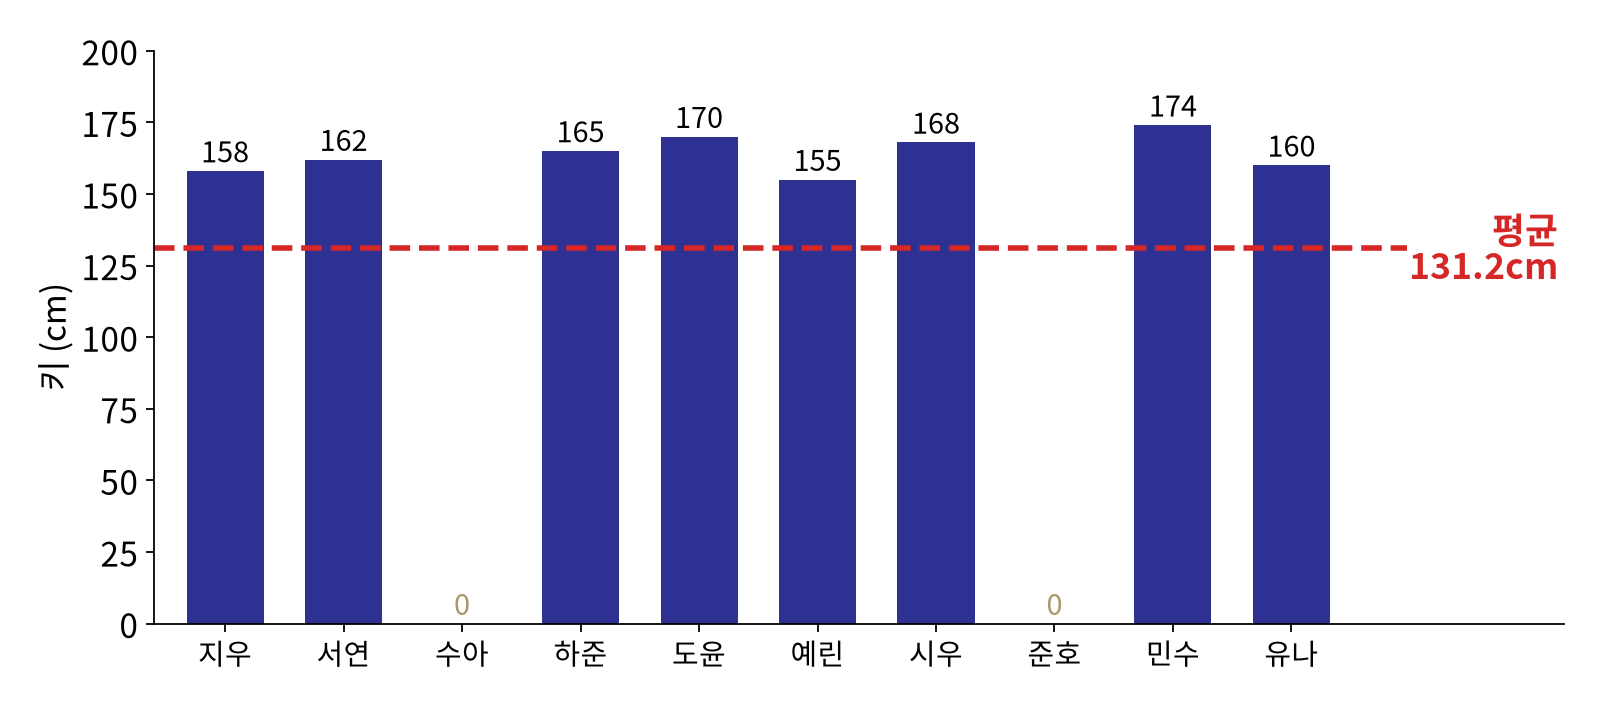
\includegraphics[width=0.74\linewidth]{dd_hook.png}\par\vskip0.3em
{\large 우리 반 10명의 키. \kq{평균 키가 131cm?} 뭔가 이상하다}
\vfill
\note{우리 반 10명의 키를 모아서 평균을 냈더니 131센티미터가 나왔습니다. 고등학생 평균 키로는 너무 작죠. 그래프를 보면 이유가 보입니다. 수아와 준호 칸이 0입니다. 키를 안 적은 두 칸에 0이 들어가서 평균을 끌어내린 겁니다. 실제 데이터에는 이런 지저분한 값이 늘 섞여 있습니다. 이걸 더티 데이터라고 하고, 오늘은 그 세 가지 모양을 배웁니다.}
\end{frame}

% --- 세 가지 모양
\begin{frame}{더티 데이터의 세 가지 모양}
\vfill
\centering
{\Large
\begin{tabular}{ccc}
\kb{① 결측치} & \kb{② 중복} & \kb{③ 이상치}\\[0.4em]
\normalsize 있어야 할 값이 없다 & \normalsize 같은 기록이 여러 번 & \normalsize 혼자 크게 튀는 값\\[0.2em]
\normalsize Missing value & \normalsize Duplicate & \normalsize Outlier
\end{tabular}}\vskip1.4em
{\large 모델을 고르기 전에, 데이터부터 본다}\\[0.4em]
{\small Garbage in, garbage out: 쓰레기를 넣으면 쓰레기가 나온다}
\vfill
\note{더티 데이터는 모양이 딱 세 가지입니다. 있어야 할 값이 없는 결측치, 같은 기록이 여러 번 들어간 중복, 혼자 크게 튀는 이상치. 아무리 좋은 모델을 써도 데이터가 더러우면 결과도 더럽습니다. 영어로 garbage in, garbage out이라고 합니다. 그래서 모델을 고르기 전에 데이터부터 봐야 합니다.}
\end{frame}

% --- 결측치
\begin{frame}{① 결측치: 0을 빼면}
\vfill
\centering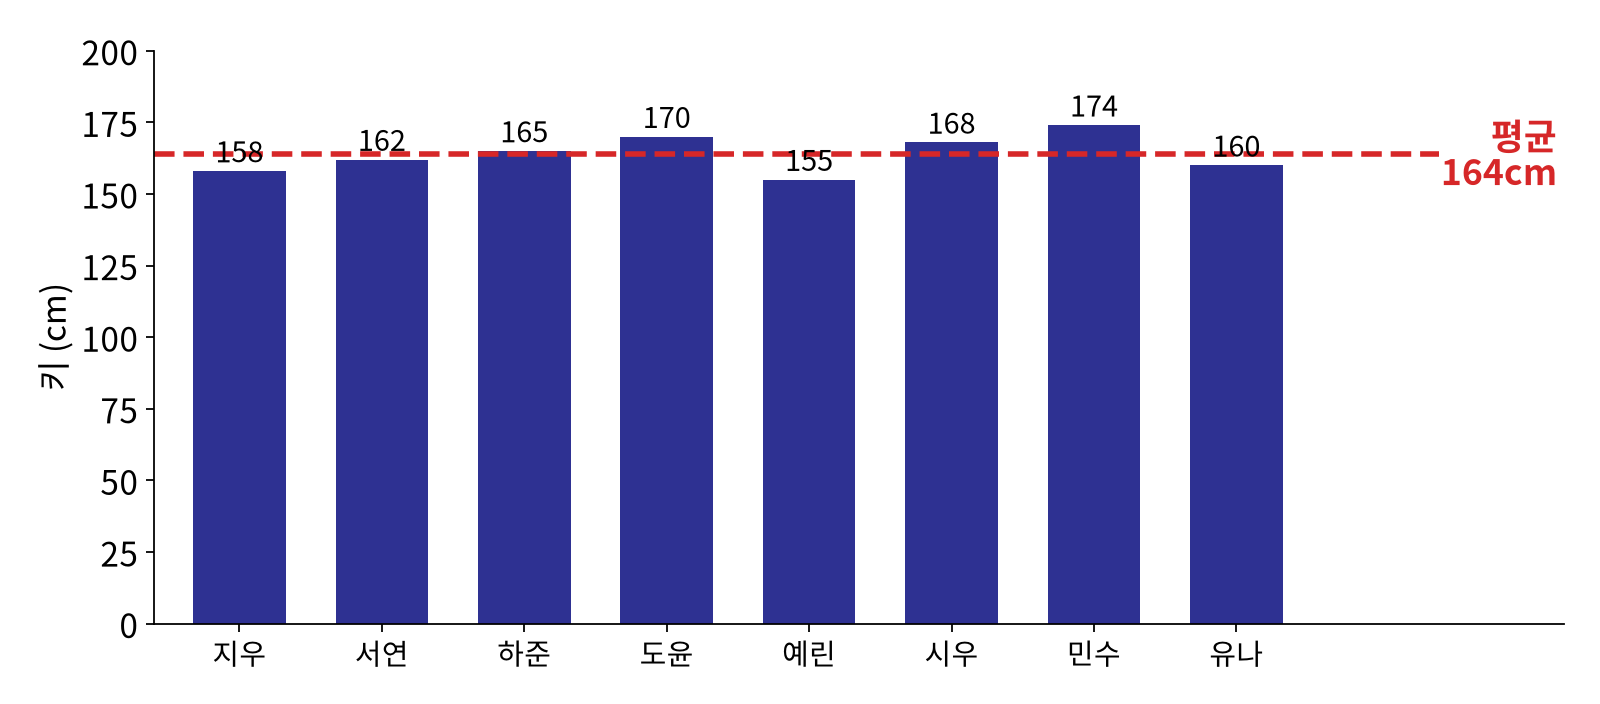
\includegraphics[width=0.74\linewidth]{dd_clean.png}\par\vskip0.3em
{\large 키를 안 적은 두 칸을 빼고 계산하면 \kb{평균 164cm}}
\vfill
\note{첫째, 결측치입니다. 수아와 준호는 키를 안 적었는데 0이 들어갔습니다. 0은 키가 아니라 비었다는 표시입니다. 이 두 칸을 빼고 8명으로 계산하면 평균 164센티미터. 훨씬 그럴듯합니다.}
\end{frame}

% --- 숫자인 척하는 결측치
\begin{frame}{숫자인 척하는 결측치가 더 위험하다}
\markpage{sentinel}
\vfill
\centering
{\Large
\begin{tabular}{lll}
\textbf{적힌 값} & \textbf{컴퓨터가 보기에} & \\[0.3em]\hline\\[-0.5em]
(빈칸) & 비었음 & \kb{눈에 띈다}\\[0.4em]
\texttt{NA}, \texttt{?} & 글자 & 계산하다 오류가 난다\\[0.4em]
\texttt{0}, \texttt{-999} & \kq{진짜 숫자} & \kq{오류 없이 평균에 섞인다}
\end{tabular}}\vskip1.0em
{\small 키 0cm, 나이 $-999$세처럼 \textbf{말이 안 되는 값}을 찾아서 빈칸으로 바꾼다}
\vfill
\note{빈칸은 눈에 띄니까 오히려 괜찮습니다. 문제는 비었다는 뜻을 숫자로 적은 경우입니다. 0이나 마이너스 999는 컴퓨터가 보기에 진짜 숫자라서 오류도 안 나고 평균에 조용히 섞입니다. 그래서 키 0센티, 나이 마이너스 999세처럼 말이 안 되는 값을 직접 찾아서 진짜 빈칸으로 바꿔야 합니다.}
\end{frame}

% --- 중복
\begin{frame}{② 중복: 같은 기록이 여러 번}
\vfill
\centering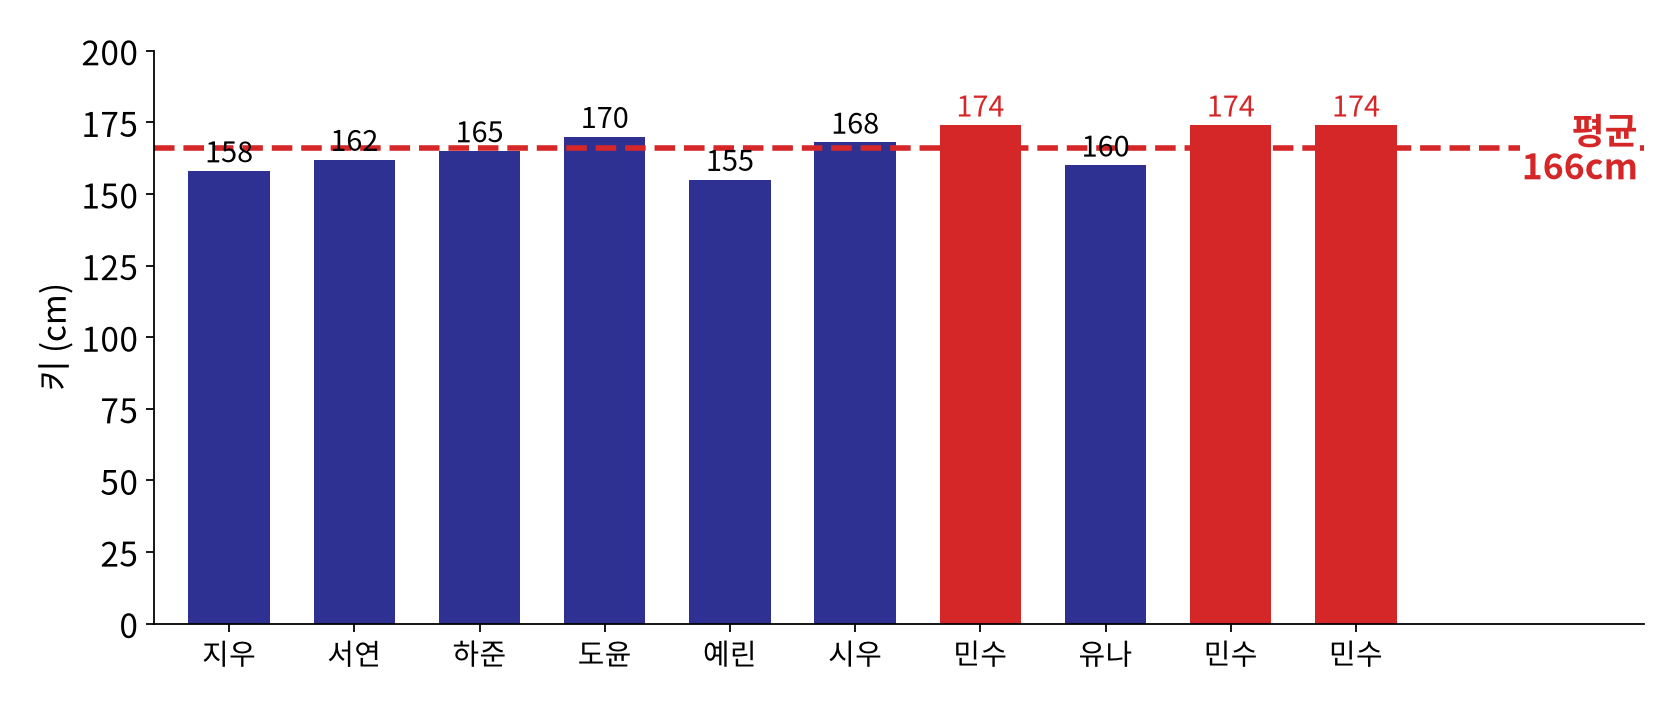
\includegraphics[width=0.76\linewidth]{dd_dup.png}\par\vskip0.3em
{\large 민수 기록이 세 번 들어가면 \kq{평균 166cm} (원래 164cm)}
\vfill
\note{둘째, 중복입니다. 설문을 여러 번 제출했거나 파일을 합치다가 같은 기록이 여러 번 들어가는 경우입니다. 키가 큰 민수 기록이 세 번 들어가면 평균이 164에서 166으로 올라갑니다. 한 사람이 세 표를 행사한 셈입니다.}
\end{frame}

% --- 같은 사람 기준
\begin{frame}{누가 ``같은 사람''인가}
\vfill
\centering
{\Large
\begin{tabular}{c@{\quad}c@{\quad}c@{\quad}l}
\textbf{줄 A} & & \textbf{줄 B} & \textbf{컴퓨터의 판단}\\\hline
\texttt{김민수, 174} & $=$ & \texttt{김민수, 174} & \kb{같은 줄: 찾는다}\\[0.6em]
\texttt{김민수, 174} & $\neq$ & \texttt{김\kq{\textvisiblespace}민수, 174} & \kq{다른 줄 (띄어쓰기)}\\[0.6em]
\texttt{김민수, 174} & $\neq$ & \texttt{김민수, \kq{171}} & 같은 사람? 동명이인?
\end{tabular}}\vskip1.0em
{\large 완전히 같은 줄은 컴퓨터가 찾지만, \kq{같다의 기준은 사람이 정한다}}\\[0.3em]
{\small 예: 이름 대신 학번으로 같은 사람을 판단한다}
\vfill
\note{완전히 똑같은 줄은 pandas의 duplicated 같은 함수가 바로 찾아 줍니다. 그런데 띄어쓰기 하나만 달라도 컴퓨터는 다른 줄로 봅니다. 이름은 같은데 키가 다르면 같은 사람이 두 번 잰 건지, 동명이인인지 알 수 없습니다. 그래서 무엇을 같은 것으로 볼지, 예를 들어 이름이 아니라 학번으로 판단할지는 사람이 정해야 합니다.}
\end{frame}

% --- 이상치
\begin{frame}{③ 이상치: 혼자 크게 튀는 값}
\vfill
\centering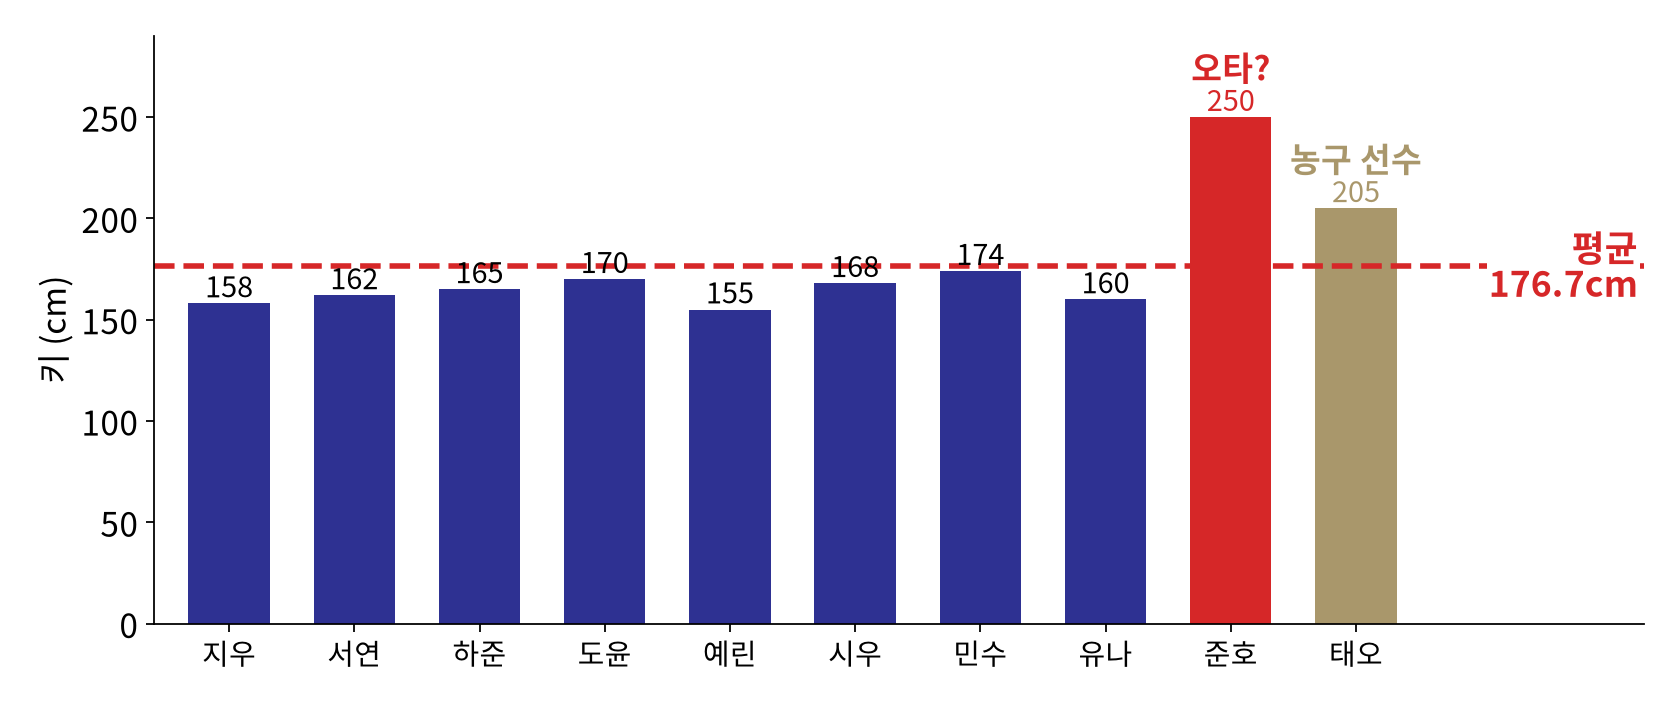
\includegraphics[width=0.76\linewidth]{dd_outlier.png}\par\vskip0.3em
{\large 준호 250cm는 \kq{오타}, 태오 205cm는 \kb{농구 선수}일 수도}
\vfill
\note{셋째, 이상치입니다. 준호의 키가 250센티미터로 적혀 있습니다. 세계 최장신 기록에 가까운 값이니 오타일 가능성이 큽니다. 이런 오타는 결측치처럼 비워 둡니다. 그런데 태오의 205센티미터는 어떨까요? 농구 선수라면 진짜일 수 있습니다. 같은 튀는 값이라도 처리 방법이 다릅니다.}
\end{frame}

% --- 그림으로 찾기
\begin{frame}{그림으로 찾는다: 상자 그림}
\vfill
\centering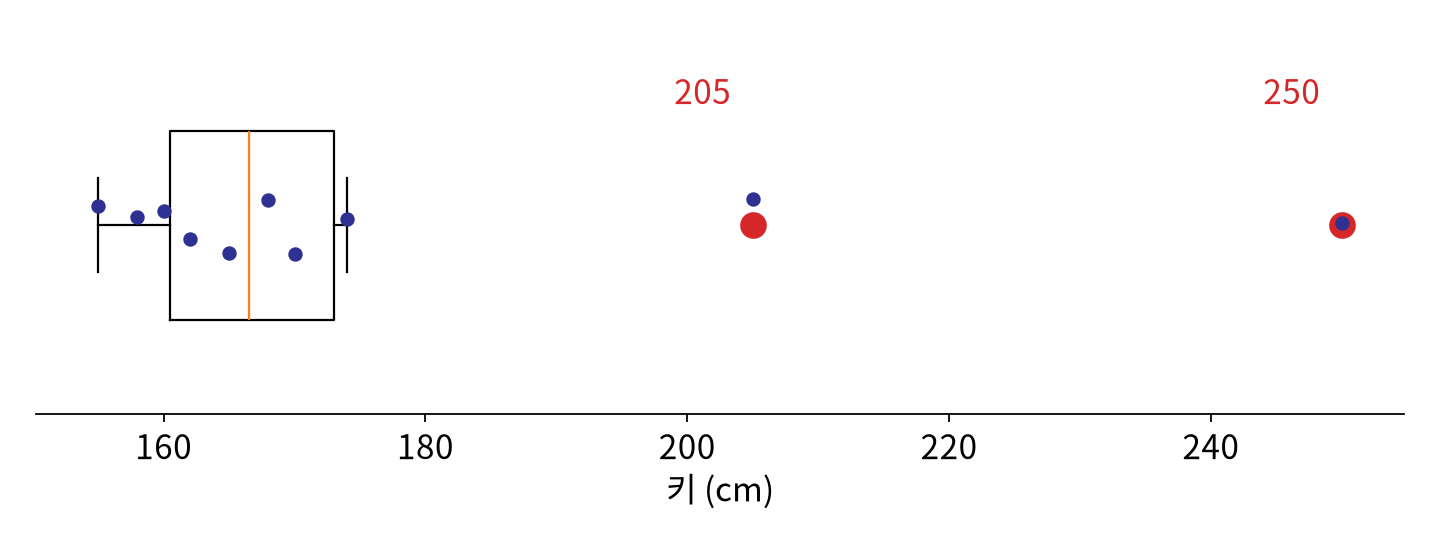
\includegraphics[height=0.62\textheight]{dd_box.png}\par\vskip0.3em
{\large 상자 = 25\%~75\% 지점(가운데 절반), 상자 속 선 = 50\%(중앙값)}\\[0.2em]
{\large 수염 = 상자 높이의 1.5배 안의 값, \kq{수염 밖에 홀로 떨어진 점}이 이상치 후보}\\[0.2em]
{\small 후보를 찾는 건 그림이, 지울지 남길지는 사람이 정한다}
\vfill
\note{이상치는 숫자 표만 봐서는 잘 안 보이고, 그림을 그리면 바로 보입니다. 상자 그림은 가운데 절반의 데이터를 상자로 그리고, 상자에서 멀리 떨어진 점을 따로 찍어 줍니다. 205와 250이 빨간 점으로 튀어나와 있습니다. 다만 그림은 후보를 알려 줄 뿐이고, 지울지 남길지는 사람이 정합니다.}
\end{frame}

% --- 지울까 남길까
\begin{frame}{지울까, 고칠까, 남길까}
\vfill
\centering
{\large
\begin{tabular}{lll}
\textbf{경우} & \textbf{예} & \textbf{처리}\\[0.3em]\hline\\[-0.5em]
분명한 오타 & 키 250cm & 빈칸으로 (결측치처럼)\\[0.4em]
단위 실수 & 꽃받침 51cm (mm 로 적음) & 고친다 ($\div 10$)\\[0.4em]
진짜일 수 있음 & 농구 선수 205cm & \kb{남긴다}\\[0.4em]
모르겠음 & ? & 표시해 두고, 지운 결과와 둘 다 보고
\end{tabular}}\vskip1.0em
\kq{판단의 근거는 그 분야를 아는 지식 (도메인 지식)}
\vfill
\note{튀는 값을 어떻게 할지 정리하면 이렇습니다. 분명한 오타는 결측치처럼 비웁니다. 단위를 잘못 적은 경우는 고칠 수 있습니다. 실습에서 보겠지만 꽃받침 길이 51은 센티미터가 아니라 밀리미터로 적은 겁니다. 진짜일 수 있는 값은 남깁니다. 정말 모르겠으면 표시해 두고 지운 결과와 안 지운 결과를 둘 다 보고합니다. 이 판단의 근거가 그 분야를 아는 지식, 도메인 지식입니다.}
\end{frame}

% --- 모델도 속는다
\begin{frame}{모델도 속는다}
\vfill
\centering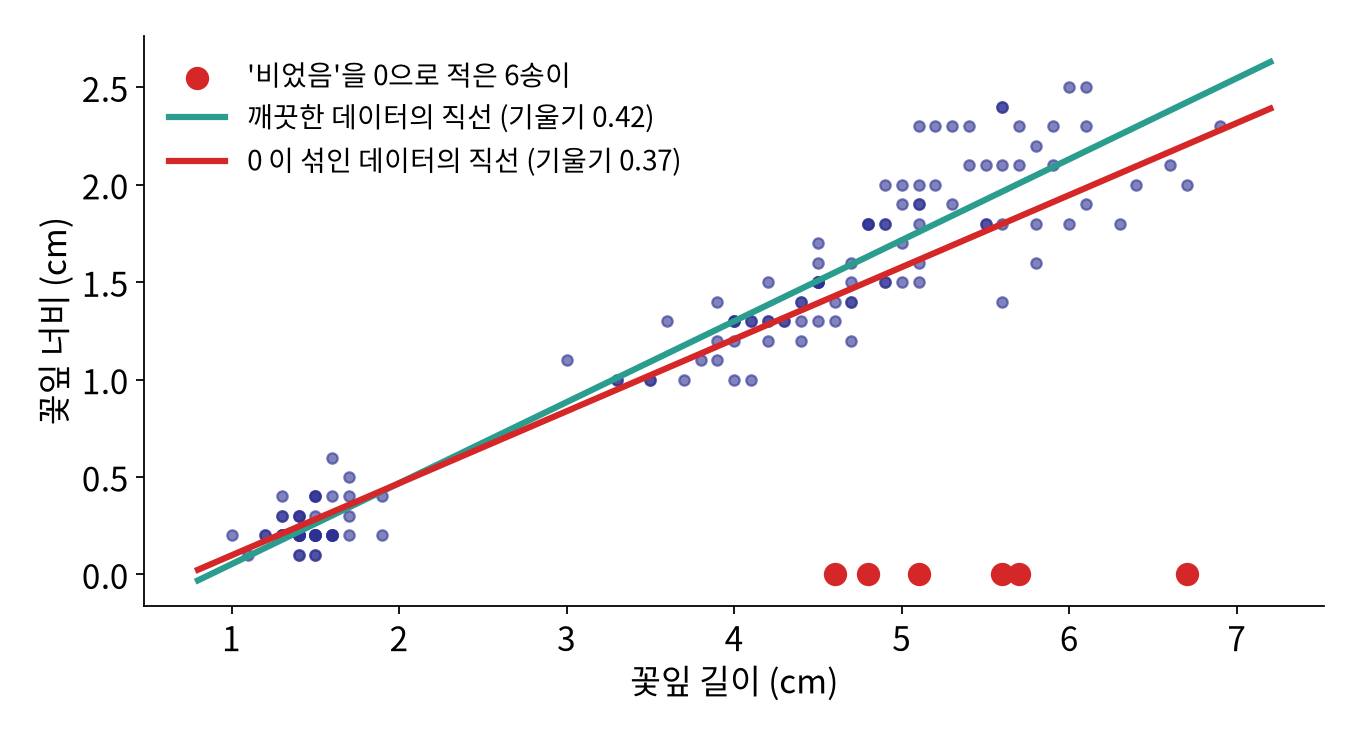
\includegraphics[width=0.66\linewidth]{dd_iris.png}\par\vskip0.3em
{\large 붓꽃 150송이 중 \kq{6송이}의 꽃잎 너비를 0으로 적었을 뿐인데, 직선이 끌려 내려간다}
\vfill
\note{더러운 데이터는 평균만 망치는 게 아니라 모델도 속입니다. 붓꽃 150송이의 꽃잎 길이와 너비입니다. 그중 6송이의 너비를 비었다는 뜻으로 0이라고 적었습니다. 초록 선은 깨끗한 데이터로 그은 직선, 빨간 선은 0이 섞인 데이터로 그은 직선입니다. 150송이 중 6송이일 뿐인데 기울기가 0.42에서 0.37로 내려갔습니다. 모델은 0을 진짜 너비로 믿고 배웁니다.}
\end{frame}

% --- 문제풀이
\begin{frame}{문제풀이}
\vfill
\begin{enumerate}
\item 키 기록 \texttt{[160, 0, 170, 0, 180]}. 평균은? 0을 결측치로 보고 빼면?\vskip0.7em
\item \texttt{"김민수"}, \texttt{"김 민수"}, \texttt{"김민수 "} 세 줄. 완전히 같은 줄 찾기로는 몇 쌍이 중복으로 잡히나? 공백을 모두 지운 뒤에는?\vskip0.7em
\item 다음 값은 오타일까, 진짜일까? 무엇을 더 알아야 할까?\\
(a) 고등학생 몸무게 450kg \quad (b) 하루 공부 시간 25시간 \quad (c) 100m 달리기 9.8초
\end{enumerate}
\vfill
\note{1번 답. 다섯 개 평균은 510 나누기 5, 102입니다. 0 두 개를 빼면 510 나누기 3, 170입니다. 2번 답. 세 줄이 모두 글자가 달라서 완전히 같은 줄 찾기로는 0쌍입니다. 공백을 모두 지우면 셋 다 김민수가 되어 셋이 모두 같은 줄, 중복이 2개 잡힙니다. 3번 답. a는 오타일 가능성이 큽니다. 45킬로그램에 0이 하나 더 붙었을 수 있습니다. b는 하루가 24시간이니 불가능한 값입니다. c는 세계 기록 근처라 고등학생이라면 의심스럽지만, 육상 선수 데이터라면 진짜일 수 있습니다. 어떤 사람들의 데이터인지를 알아야 합니다.}
\end{frame}

% --- 실습
\begin{frame}[fragile]{실습: 지저분한 iris 청소하기}
\vfill
\centering\begin{tabular}{rl}
\large 0 & 일부러 더럽힌 붓꽃 데이터를 받아 \texttt{describe()} 로 훑어보기\\[0.5em]
\large 1 & 결측치: 빈칸 $\cdot$ 0 $\cdot$ $-999$ 를 찾아 진짜 빈칸으로\\[0.5em]
\large 2 & 중복과 표기: \texttt{'Setosa'}, \texttt{' setosa'} 맞추기 $\to$ 숨은 중복 찾기\\[0.5em]
\large 3 & 이상치: 상자 그림으로 51cm 꽃받침 찾아 고치기\\[0.5em]
\large 4 & 청소 전 vs 후: 같은 모델의 정확도 \kq{86\%} $\to$ \kb{96\%}
\end{tabular}\vskip1em
Iris (붓꽃 150송이, scikit-learn 내장) \\[0.4em]\href{https://colab.research.google.com/github/SuminHan/book-ml/blob/main/slides/v2/ml1/week01/dirty_data/lab/dirty_data.ipynb}{\textcolor{ksagolddk}{▶ Colab에서 실습 노트북 열기}}
\vfill
\note{실습에서는 붓꽃 데이터에 제가 일부러 더러운 값을 섞어 뒀습니다. 빈칸, 0, 마이너스 999, 대소문자와 공백이 섞인 꽃 이름, 중복된 줄, 밀리미터로 적은 꽃받침 길이. 이걸 하나씩 찾아서 고칩니다. 마지막에는 청소하기 전과 후의 데이터로 같은 모델을 학습시켜 봅니다. 청소 전에는 꽃 종류가 3개가 아니라 8개로 잡히고 정확도가 86퍼센트인데, 청소하면 원래 깨끗한 데이터와 같은 96퍼센트가 됩니다.}
\end{frame}

% --- 정리
\begin{frame}{정리}
\vfill
\centering\large\begin{tabular}{l}
결측치 \quad 빈칸보다 \texttt{0}, \texttt{-999} 처럼 숫자인 척하는 값이 더 위험\\[0.5em]
중복 \quad 완전히 같은 줄은 컴퓨터가, ``같다''의 기준은 사람이\\[0.5em]
이상치 \quad 그림으로 찾고, 오타인지 진짜인지는 도메인 지식으로\\[0.5em]
모델도 속는다 \quad 모델을 고르기 전에 데이터부터 본다
\end{tabular}
\vfill
\note{정리합니다. 결측치는 빈칸보다 0이나 마이너스 999처럼 숫자인 척하는 값이 더 위험합니다. 중복은 완전히 같은 줄은 컴퓨터가 찾지만, 무엇이 같은지 기준은 사람이 정합니다. 이상치는 그림으로 찾고, 오타인지 진짜인지는 도메인 지식으로 판단합니다. 그리고 더러운 데이터는 모델도 속입니다. 모델을 고르기 전에 데이터부터 보세요. 여러분이 학기 프로젝트에서 데이터를 받으면 가장 먼저 할 일이 이겁니다.}
\end{frame}
\end{document}
